\documentclass[48pt,spanish]{article}
\usepackage[utf8]{inputenc} 	%Define tildes las tres siguiente lineas
\renewcommand{\baselinestretch}{3.5} 
\usepackage[landscape,a4paper]{geometry}
\geometry{verbose,tmargin=2cm,bmargin=2cm,lmargin=2cm,rmargin=2cm}  
\usepackage{graphicx}
\usepackage{shadowtext}
\usepackage{eso-pic}
\usepackage{xcolor}
\usepackage{mathptmx}
\usepackage[11pt]{moresize}

\xdefinecolor{grafitohatari}{rgb}{1,1,1}
\graphicspath{{Png/}}


%---------------figuradefondo--------------------------------
\newcommand\BackgroundPic{
\put(-3,0){
\parbox[b][\paperheight]{\paperwidth}{%
\vfill
\centering
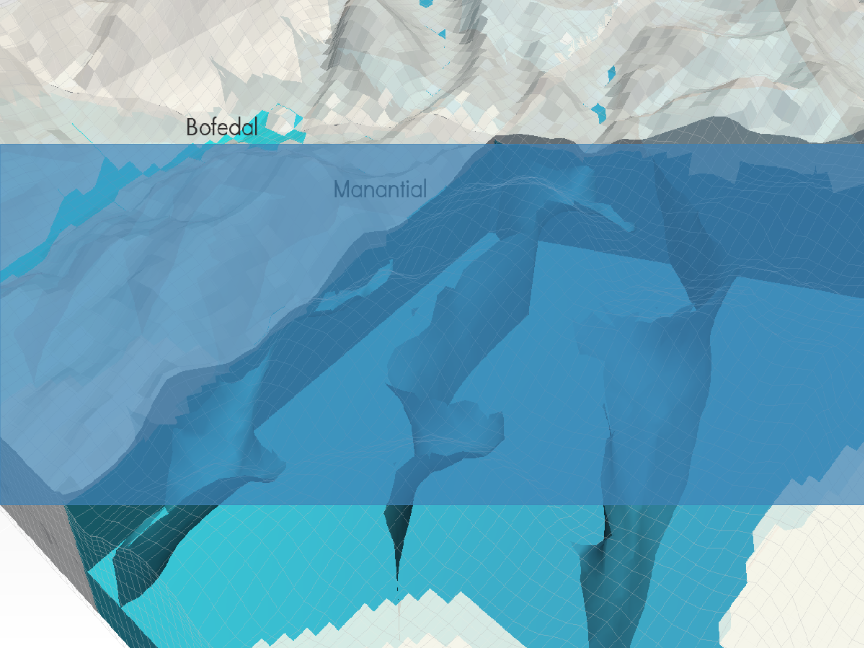
\includegraphics[width=\paperwidth,height=\paperheight]{Input/imagen.png}% 
\vfill
}}}
\AddToShipoutPicture*{\BackgroundPic}



%---------------tipo de letra--------------------------------


%\usepackage[sfdefault]{cabin}
\usepackage{lmodern}
%\renewcommand*\ttdefault{lmvtt}
\usepackage[T1]{fontenc}
\newcommand*{\myfuentechica}{\ttfamily\slshape\fontsize{36}{40}\selectfont}
\newcommand*{\myfuentegrande}{\ttfamily\mdseries\fontsize{40}{48}\selectfont}
\newcommand*{\myfuentedetalles}{\ttfamily\slshape\fontsize{24}{30}\selectfont}
\newcommand*{\mysombra}{\shadowcolor{{RGB}{255,51,76}} \shadowoffset{2pt}  }



%---------------comienzo--------------------------------
\begin{document}
\color{grafitohatari}




\vspace*{\fill}
\center


{\myfuentegrande \mysombra  \shadowtext {Seminario 13 Febrero}}\\
{\myfuentegrande \mysombra  \shadowtext {Modelamiento Numérico de Bofedales}}\\
{\myfuentegrande \mysombra  \shadowtext {y Manantiales y Evaluación del Impacto}}\\
{\myfuentechica  \mysombra \shadowtext {de la Minería}}\\


\begin{flushright}

\includegraphics [scale=0.3, angle=25]{Logo/gidahatari.png}       \\
\end{flushright}

\vspace*{\fill}



\end{document}
